
%%%%%%%%%%%%%%%%%%%%%%% file typeinst.tex %%%%%%%%%%%%%%%%%%%%%%%%%
%
% This is the LaTeX source for the instructions to authors using
% the LaTeX document class 'llncs.cls' for contributions to
% the Lecture Notes in Computer Sciences series.
% http://www.springer.com/lncs       Springer Heidelberg 2006/05/04
%
% It may be used as a template for your own input - copy it
% to a new file with a new name and use it as the basis
% for your article.
%
% NB: the document class 'llncs' has its own and detailed documentation, see
%
%
%%%%%%%%%%%%%%%%%%%%%%%%%%%%%%%%%%%%%%%%%%%%%%%%%%%%%%%%%%%%%%%%%%%


\documentclass[runningheads,report]{llncs}

\usepackage{amssymb}

\setcounter{tocdepth}{3}
\usepackage{graphicx}
\usepackage{multirow}%使用多栏宏包

\usepackage{url}
\urldef{\mailsa}\path|songleyi@student.ecnu.edu.cn|
\newcommand{\keywords}[1]{\par\addvspace\baselineskip
\noindent\keywordname\enspace\ignorespaces#1}

\begin{document}

\mainmatter  % start of an individual contribution

% first the title is needed
\title{ClickKeeper: A Framework of  Malicious Click Prevention and Detection
\thanks{The first term thesis proposal aborted due to the sudden switch towards the click fraud detection application problem of mine. I've done some survey work on computational advertising ecosystem and thought up a reasonable framework and flow of ad server core. All is about ad serving and ad selection. But searching a decent experiment stucks me.  Considered my task buckets and semester schedule, it might only be hopefully if I changed my direction and make the report more close to the works recently read.
}
}

% a short form should be given in case it is too long for the running head
\titlerunning{ClickKeeper: A Framework of Malicious Click Prevention and Detection}

% the name(s) of the author(s) follow(s) next
%
% NB: Chinese authors should write their first names(s) in front of
% their surnames. This ensures that the names appear correctly in
% the running heads and the author index.
%
\author{Leyi Song}
%
\authorrunning{ClickKeeper: A Framework of Malicious Click Prevention and Detection}
% (feature abused for this document to repeat the title also on left hand pages)

% the affiliations are given next; don't give your e-mail address
% unless you accept that it will be published
\institute{Software Engineering Institute,\\
East China Normal University,\\
Shanghai, China\\
\mailsa\\}

%
% NB: a more complex sample for affiliations and the mapping to the
% corresponding authors can be found in the file "llncs.dem"
% (search for the string "\mainmatter" where a contribution starts).
% "llncs.dem" accompanies the document class "llncs.cls".
%

\toctitle{Lecture Notes in Computer Science}
\tocauthor{Authors' Instructions}
\maketitle


\begin{abstract}
Advertising plays a vital role in supporting free websites and smartphone apps. Fraudulent advertising click activities linked directly to the flow of money in online advertising. Reputed online ad networks or servers is responsibe for the detection of click-spams. In our work, we proposed our click fraud detection framework and techniques, including offline classifier-based method and online duplicate detection. We then focus on the duplicate click detection on click stream of sliding window models. The TBF(Timing Bloom Filter) algorithm was implemented and applied for the duplicate click detection on the datasets. The experiments show that our approaches give resonable methodologies and technical framework for solving malicious click detection problems. 
\keywords{Click Fraud; Computational Advertising; Data Stream; Duplicate Detection}
\end{abstract}

%%%%%%%%%%%%%%%%%%%%%%%%%%%%%%%%%%%%%%%%%%%%%%%%%%%%%%%%%%%%%%%%%%%%%%
%%%%%%%%%%%%%%%%%%%%%%%%%%%%%%%%%%%%%%%%%%%%%%%%%%%%%%%%%%%%%%%%%%%%%
\section{Introduction}

Online Advertising has been a vast ecosystem on the web sustains numerous free websites and 
smartphone apps. All roles, including advertiser,web user and website publisher can own  profit from advertising. Then, the economic system  arise with the advertising ecocsystem, as well as the fraudulent activities in the network.

Click-fraud, i.e., click spam, malicious click or invalid click(called in Google) on online ads where the user has no actual interest in the advertiser's site, results in advertising revenue being misappropriated by click-spammers\cite{DBLP:conf/sigcomm/DaveGZ12}.

Since online advertising networks, such as Google, act as brokers of multi-billion dollar online advertising revenue streams, click fraud is a major responsibility and concern\cite{kintana2009goals}. Nowadays, reputed online ad networks have in-house heuristics to detect click-fraud and discount these clicks\cite{website:GoogleReport}. However, it is not clear any heuristic is perfect. Advertisers have to pay for false negatives (click-spam missed by the heuristic).

In other cases, addressing fraudulent clicks in clickthrough data is necessary for the next step analysis on the log data, as the malicious noise in click log will influence the results of CTR(Click-through rate) prediction in search engines or advertising servers.

\subsection{Motivation}

Click frauds put threats to the lucrative search engine market. Threats to the search engines' underlying business model are also threats to the free services that provide to millions of users, making click fraud a concern for all\cite{DBLP:journals/computer/Jansen08}. 

In the CPC(Cost-per-click) market, the existing research on traffic quality or malicicous click detection is insufficiently visible to others, including lots of in-house algorithms.  However, click fraud problem heavily challenges the CPC model: the ad link is clicked without actual advertising impression. A survey indicates that Internet advertisers paid \$0.8 billion for click fraud in 2005 and \$1.3 billion estimated in 2006, and about 14.6\% clicks are fraudulent\cite{website:HotTopics}.

As state previously, there have been few systematically prevention and detection systems open to us. For all these reasons, we propose a feasible and effective framework of the click-spam filtering flows. Above of all, an important issue in defending click fraud is how to deal with duplicate clicks. Even if it is very difficult to identify which scenario the identical clicks belong to, it is surely reasonable that prescribe the identical clicks will not count if they are within short time interval. In this paper, we present one part of the online detection methods, which involves the duplicate click detection on pay-per-click streams using sliding window model.


\subsection{{Decaying Window Models on Stream}}

Decaying window models can be utilized to eliminate expired information. There are two common types of decaying windows: count-based windows which maintain the last (most recent) N items in the data stream, and timebased windows which maintain all items that arrived in the last T time units. Therefore, the time span of a count-based window may vary, while the number of items in a timebased window may change from time to time\cite{DBLP:conf/icdcs/ZhangG08}. Our methods based on the count-based windows, however it is easy to migrate to the other case.

\subsubsection{Sliding window:}
A sliding window, first introduced by Datar et al.\cite{DBLP:conf/soda/DatarGIM02}, only contains the last N items, which is updated once a new element comes and an old element expires. Since the elements in a sliding window expire one by one, usually some timing information is maintained to update the interested statistics when the window slides.

There are other kinds of decaying window models: landmark window and jumping window. In our experiments, we will just use sliding window which is more applicable in the click log online analysis case. It also can be found in \cite{DBLP:conf/icdcs/ZhangG08} that jumping windown can be easily extended to adopt the algorithms.

\subsection{Our Contribution}
There are three main contributiong we made in this work: 1) We present a feasible and effective framework of malicious click detection and prevention system flows. 2) We adopt TBF(Timing Bloom Filter) algorithm in \cite{DBLP:conf/icdcs/ZhangG08} in click stream for duplicate click detection. The algorithm is extented and implemented reasonably. 3) Under our online framework part-of implementation, we practise on real data and make a comparision with ideal synthetic data. In conclusion, we give much details about detecting techniques which can be adopted by others and the research can be future expaned with more inventive data structure and algorithms. 


\subsubsection{Roadmap}

The rest of the paper is organized as follows. Section 2 highlights the related work. We first suvey on the existing or on-going click fraud detection researches and techniques. We consider detail on the problem of detecing online click stream. \texttt{ClickKeeper} - A framework for malicious click detection is given in Section 3. We introduce the general online and offline methods adapted to our framework. To detect duplicate clicks over sliding window, bloom filter basic data structure and TBF algorithms are introduced in Section 4. In section 5, we make a abstract analysis on TBF applied in our cases. We evaluate our algorithm implementation and experiment it on synthetic datasets and real datasets in Section 6. We finally conclude and discuss our future work in Section 8 and Section 9.

%%%%%%%%%%%%%%%%%%%%%%%%%%%%%%%%%%%%%%%%%%%%%%%%%%%%%%%%%%%%%%%%%%%%%%%%%%%%
%%%%%%%%%%%%%%%%%%%%%%%%%%%%%%%%%%%%%%%%%%%%%%%%%%%%%%%%%%%%%%%%%%%%%%%%%%%
\section{Related Work}

The malicious click annoys the online advertising ecosystem for a few years. Since \texttt{Lane's Gift and Collectibles} filled a law suit against Google on behalf of all Google advertisers about click fraud in 2005, Google askeded Alexander Tuzhilin to evaluate Google invalid click detection efforts in Mid 2006. Then, based on Google's internal click fraud recognizing systems and in-house algorithms, a report about invalid click filtering \cite{website:GoogleReport} was open to industry.

Fraudulent Activities pervades any information system, be it e-mail or web, social, blog or reviews platform. Spirin and Han in \cite{DBLP:journals/sigkdd/SpirinH11} categorized and demonstrated the scope of various web spam problem and existing solving algorithims. In this web spam taxonomy, click spam means in two aspects: one aims to push "malicious noise" into a query log with the intention to corrupt data, the other means the click fraud activities we have talked in advertising environment. No matter what kind of click fraud, the work in \cite{DBLP:conf/wsdm/YuXK10} about the detection of click bot traffic can benefitting both.

Except click bots, click fraud's source varies from mannual click to publiser's malicious page scripts. Therefore, there should be a systematic prevention and detection methods for click frauds. In \cite{DBLP:journals/ccr/Haddadi10}, they provides an incentive approaches to distinguish botnets and benigh human. This kind of special ads, called \textit{bluff ads}, which use the bluff/real ratio of the user's browsing experience to address different forms of click-fraud attacks.

The online advertising providers, such as ad network and ad exchange, also make their efforts to detecting the real-time click behaviors. Metwally, A. et al make their effort on online advertising stream analysis.In their work \cite{DBLP:conf/www/MetwallyAA07}, they built on several published theoretical results to devise the \textit{Similarity-Seeker} algorithm that discovers coalitions made by pairs of fraudsters. In \cite{DBLP:conf/vldb/MetwallyAA05} they develop an algorithm, Streaming-Rules, to report association between pairs of elements in streams. Especially, a solution based on Bloom Filters was developed in \cite{DBLP:conf/www/MetwallyAA05}, and the proposed algorithm runing in both the contexts of sliding, and landmark stream windows. The work \cite{DBLP:conf/icdcs/ZhangG08} which contains \texttt{Timing Bloom Filter} is a better modification of Bloom Filter in stream duplicate detection.


In most cases, fraudulent clicks are detected offline from click logs. Google's approaches in \cite{website:GoogleReport} show that they use several filters for invalid clicks detect, which are anomaly-based, rule-based and classifier-based respectively. Classification approaches are always useful in the situation. The system described in \cite{Martin:Thesis:2010} builds a number of classifiers, which includes classification trees, association rule, support vector machines, Bayesian classification and outlier detection methods. In this system, they integrated with the former system and experimented their classifiers and choose some well-output models to have next refinement. So far, after discussing kinds of malicious click prevention and detection methods, it is hard to see a entirely systematical detection framework, as well as detailed techinques and experiments. Therefore, it is valuable to have a reasonable framework of click fraud detection.

%%%%%%%%%%%%%%%%%%%%%%%%%%%%%%%%%%%%%%%%%%%%%%%%%%%%%%%%%%%%%%%%%%%%%%%%%%%%%%%
%%%%%%%%%%%%%%%%%%%%%%%%%%%%%%%%%%%%%%%%%%%%%%%%%%%%%%%%%%%%%%%%%%%%%%%%%%%%%

\section{ClickKeeper: Overview of Our Approach}
Given an ad serving system, no matter it is in an ad network or an ad exhange, malicious click detection and prevention can be integreted in many sub-parts. Therefore, we sketch a two part click fraud detection system, called \texttt{ClickKeeper}.

\subsection{Architecture}

In our approaches, there are mainly two seperated stages, \texttt{online process} and \texttt{offline analysis}. Firstly, the online stage process the click logs in streams, then duplicate detection and other preprocessing methods are applied. In the offline analysis stage, malicious clicks are addressed by classifiers, then a blending strategy combines the results to ensure the false positive rate in a given range.



The steps in each stage can be extended or modified in our framework. The sketch of our apprpaches is shown in figure 1. There are several steps in both offline and online stage. 



\subsubsection{Online stage.}
The online stage is like a mediator between the ad serving module and the click logging module. There should be a API from the serving system and catch the click log flow from the network. The process considered to be in a short time. The stream go through duplicate detection filter and other rule-based filters, coming finally to the format processor. Output formatted click logs without some piece of invalid clicks to the ad log system.

\subsubsection{Offline stage.}
The offline stage is doing some analysis on the ad logs, on the output of online stage processors. The simple model is a bunch of classifiers, filters an filters. It may include the outlier method based filters, such as Z-score, and the classification method filters, such as Naive Bayes, Random Forest and SVM.  

\begin{figure}
\centering
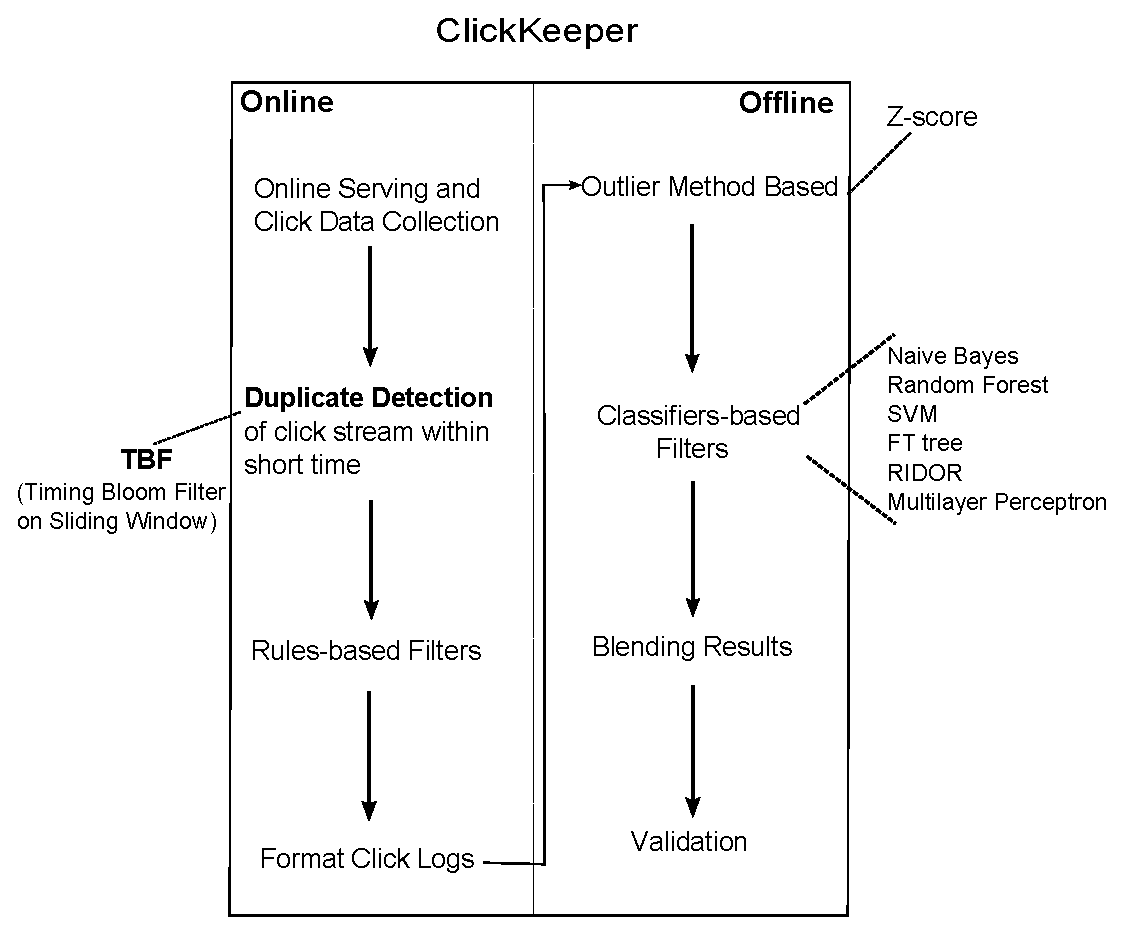
\includegraphics[height=10.5cm]{pic/clickKeeper}
\caption{ClickKeeper architecture, including online stage and offline stage. Online processor is in charge of the stream filtering of duplicate and other anti-rule clicks, prevent them go into logs. Offline is in charge of malicious click noise mining and addressing.}
\label{fig:clickKeeper}
\end{figure}



\subsection{Offline Mehods}
In our approache, we choose classification algorithms as our offline methods to build our classifiers from a set of training data.

One advantage with a classification approach is that once a model for classification has been built, the classification of instances is usually quite fast. Instance classification can also be easily distributed, as classifier instances on separate nodes in a cluster can work on copies of the model and subsets of the dataset\cite{Martin:Thesis:2010}. The classification methods analysis phrase could be work like in figure 2. The input is some well-selected attributes in click logs. And, there are some classification models to train and filter the log with their output being refinement with input operators.


The classification algorithms have many categorizations. If the system is implemented on real systems, it is better to test more methods and choose the bests. However, in present, the offline stage analysis will have detailed research in our future work.


\begin{figure}
\centering
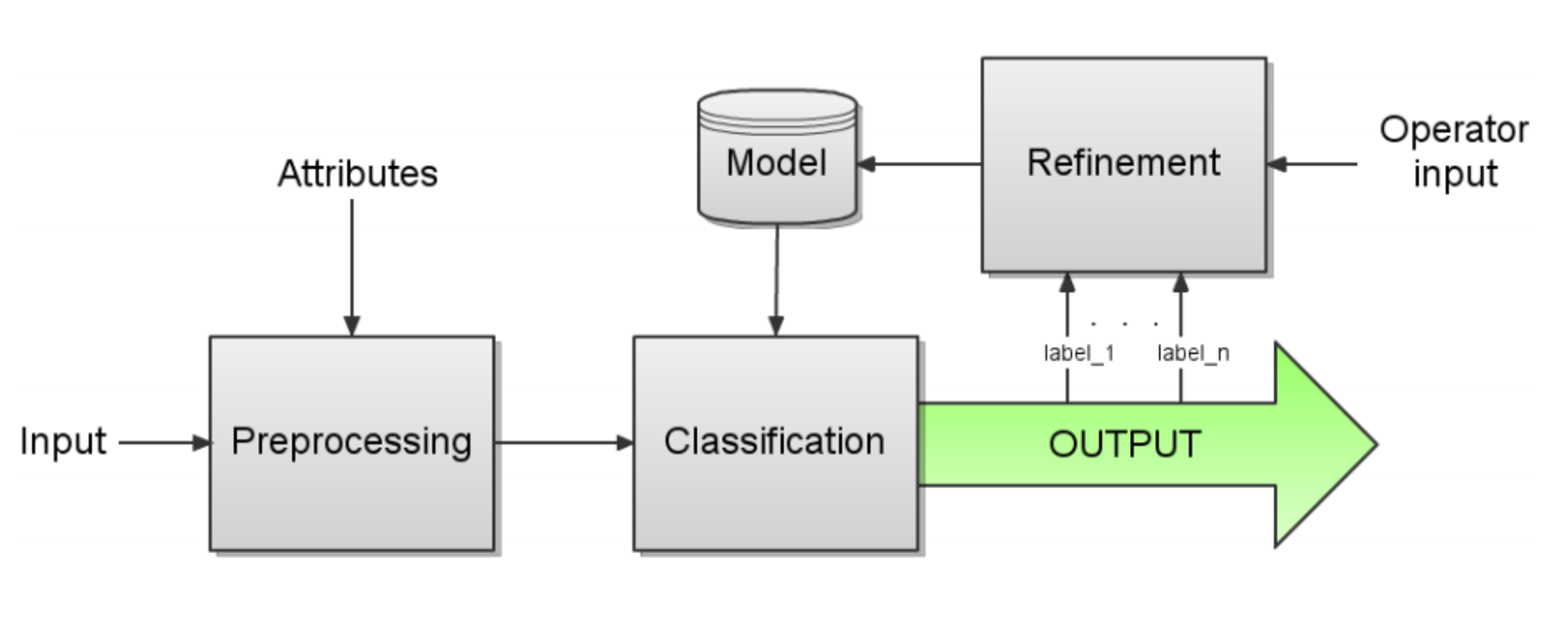
\includegraphics[height=4.8cm]{pic/classifier}
\caption{Offline detection(based on classification methods) referenced system architecture}
\label{fig:classifier}
\end{figure}

\subsection{Online Methods}

Google's approach gives us  many suggestions\cite{website:GoogleReport}. In the following, we will have a review of its online filtering methods and mixed with our adopted scheme.

\subsubsection{Rule-based online filters.}

Each rule has one or several conditions in its antecedent and is of the form “IF Condition1 AND Condition2 AND … AND ConditionK hold THEN Click X is Invalid (or respectively Valid).” An example of such a rule is “IF Doubleclick occurred THEN the second click is Invalid.” These rules are specified by invalid click detection experts based on their experiences. Therefore, these experts define what valid and invalid clicks are.

These rule-based filters  monitor various logs for certain conditions and check if the clicks in these logs satisfy these conditions. Moreover, some of the filters are not only rule-based, but also anomaly-based because the conditions of some of these rule-based filters check for certain anomalous behaviors.  

\subsubsection{Online filtering in short time.}

The filtering process is done online, meaning that the detection of an invalid click should take place within a short time window since that click occurred. For this reason and because of the never-seizing arrivals of new clicks, the detection process should be efficient and scalable to very large volumes of clicks.  

One of the online rule-based filtering problem is duplicate click detection techniques in short period of time. We can formalize the problem to duplicate detection on data stream, which will depend on the way the stream is handled.  Duplicate clicks detection within a short period of time, 10 minutes for example,  challeges our stream analysis strategy.  We will emphasis on these discussions in the following sections.



\subsection{Performance of filters}

Before presenting the methods and results,  we will show some evaluation methods. In data mining and related disciplines, there exist many measures determining performance of data mining models. One of the most popular ones is the confusion matrix that is defined as follows in table 1.

 \begin{table}[htbp]
\centering
\caption{Confusion matrix for evaluation}
\begin{tabular}{cc|c|c}
\cline{3-4}
\multirow{2}{*}{} & \multirow{2}{*}{ } &  \multicolumn{2}{|c}{\emph{Click classified by filters}} \\
\cline{3-4}
& & Invalid & Valid \\
\hline
\multirow{2}{*}{\emph{Actual click} \ } &  \multicolumn{1}{c|}{Invalid \ }  &  \multicolumn{1}{|c}{True Positive}  &  \multicolumn{1}{|c}{False Negative} \\
\cline{2-4}
 &  Valid \  & False Positive  &  True Negative \\
\hline
\end{tabular}
\end{table}

More details about the measurements show below.
\begin{equation}
TPR(True\ Positive\ Rate) = \frac{{true\ positives}}{{true\ positives + false\ negatives}}\
\end{equation}
\begin{equation}
FPR(False\ Positive\ Rate) = \frac{{false\ positives}}{{true\ negatives + false\ positives}}\
\end{equation}
\begin{equation}
TNR(True\ Negative\ Rate) = \frac{{true\ negatives}}{{true\ negatives + false\ positives}}\
\end{equation}

\begin{equation}
ACC(Accuracy) = \frac{{true\ positives + true\ negatives}}{{all\ ins\tan ces}}\
\end{equation}
\begin{equation}
{A_{ROC}}({\mathop{\rm Re}\nolimits} ciever\ Operating\ Characteristic\ Area)\
\end{equation}


%%%%%%%%%%%%%%%%%%%%%%%%%%%%%%%%%%%%%%%%%%%%%%%%%%%%%%%%%%%%%%%%%%%%%%%%%%%%%
%%%%%%%%%%%%%%%%%%%%%%%%%%%%%%%%%%%%%%%%%%%%%%%%%%%%%%%%%%%%%%%%%%%%%%%%%%%%%%
\section{Duplicate Detection of Online Filter}
Although the definition of malicious is quite obscure, a reasonable countermeasure is to prescribe that identical clicks will not count if they are within a short time interval. Then, the imoortant issue is how to detect and deal with duplicate clicks. Most traditional duplicate detecting algorithms over different decaying window, especially the sliding window still lacks efficient and effective solutions. One popular data structure for duplicate detecting is Bloom Filter. We will apply one variation of Bloom Filter in our case.
\subsection{Classical Bloom Filter}

Bloom Filter were presented by Burton H. Bloom \cite{DBLP:journals/cacm/Bloom70} in 1970, and have been widely utilized in many areas such as networking and database\cite{DBLP:journals/im/BroderM03}.  A Bloom Filter is a space-effcient data structure for representing a set of n elemnts to respond membership queries. It is a vector of m bits which are all initialized to value 0. Given a query whether an element is present in the Bloom filter, this element is hashed using the same k hash functions and the Bloom filter is checked whether all the corresponding bits are set to 1. If any one of them is 0, then undoubtedly this element is not in the dataset; otherwise, we would say that it is present in the dataset, although there is a certain probability that the element is falsely determined to be in the dataset while it is actually not. Such false cases are called false positives. 


The space-efficiency of Bloom filters is achieved at the cost of small acceptable
false positive rate f . Suppose that n distinct elements are
inserted into the Bloom filter, from \cite{DBLP:conf/sigcomm/FanCAB98}, the false positive
rate is $f = {(1 - {(1 - {1 \over m})^{kn}})^k} \approx {(1 - {e^{ - {{kn} \over m}}})^k}$ . When m and n are given, f is minimized when $k = \ln 2 \times {m \over n}$. Thus,
we have $f \approx {2^{ - k}} \approx {0.6185^{{m \over n}}}$ \cite{DBLP:conf/icdcs/ZhangG08}.

\subsection{Timing Bloom Filter}


Timing Bloom Filters data structure are proposed in \cite{DBLP:conf/icdcs/ZhangG08} which contains timing information derived from classical Bloom Filters(also introduced below)\cite{DBLP:journals/cacm/Bloom70} . 


The aim is to solve the deletion of expired data in Bloom Filter. In sliding window, although we can keep N Bloom Filters, each of which only hold one element with its winodow, maintaing N Bloom Filters makes the running time unacceptable when the window size is big. The timing information contained in TBF can be utilized to evict stale data out of the data structure, and make TBF applicable to process data streams over sliding windows.


Let N denote the sliding window size. An existing element is called \textit{active} if it is one of the most recent N elements within the current window, or \textit{expired} if it left the current window. For each element \texttt{x}, an index \texttt{pos} is used to record its timestamp in the data stream, which is an indicator of ``active`` or ``expired`` by comparing with \texttt{pos} - the index of the most recent element\cite{DBLP:conf/icdcs/ZhangG08}.


\begin{figure}
\centering
\includegraphics[height=4.6cm]{pic/TBFnew}
\caption{Example TBF data structure. In the TBF contains the hased entries of M=7 elements in the current sliding window. Each of the entrie contains the timestamp of the most recently hased element's timestamp.}
\label{fig:example}
\end{figure}


\subsection{TBF in practice}

We use the TBF data structure above in our application. Figure 3 shows an example of TBF structure with \textit{Windows size} = 7. To insert timing information into TBF, each bit in the classical Bloom Filter is replaced by an entry with $O(\log N)$ bits. In our cases, the all bits in the bit set which contains the TBF entries are initialized to bit 0. When a new element arrives, we calculate the $k$ hash functions and get $k$ indices. Then check the corresponding $k$ entries if the elements in them is both present\footnote{Present - means no entry in the k corresponding entries is all 0s.} and active\footnote{Active - means all timestamps in these k corresponding entries are within the current sliding window.}. If it is present and active, then we just ignore it and report it as a duplicate click; otherwise, we set the corresponding k entries using the element's timestamp\cite{DBLP:conf/icdcs/ZhangG08}.


To bound the bits to represent the timestampe in the continuous click stream, we use wraparound counters, with maximum N and minimum 1, that is, the $N+1$-th element's timestamp is 1 instead of $N+1$. When a new element arrives with timestamp P, there are two steps to process our algorithm. \textbf{Step 1} delete expired information in TBF, in sliding window, to clear the old element corresponding entries with timestamp P is needed. \textbf{Step 2} process the new element and add its timing infomation to the corresponding TBF entries. Therefore, besides processing the new arriving element, the expired timestamps in the TBF must be removed, which means TBF algorithm only maintains the timestamps of active elements in the current window.

%%%%%%%%%%%%%%%%%%%%%%%%%%%%%写到这里了  该写TBF的详细操作介绍了  2013-1-6  %%%%%%%%%%%%%%%%%%%%%
Figure 4 and figure 5 shows the operations when a new element comes in sliding window. In the example, we consider the scenario that we set our windows size with 7 and predefine two hash function use MD5 or SHA1 or other hash functions. 

\begin{figure}
\centering
\includegraphics[height=4.6cm]{pic/delete}
\caption{When a new element comes, we should delete the expired elements first. In this case, the element with the same wraparound timer of new comes, that is t=3, should be deleted. To find out which entries it has been hashed, the timing information make it possible. The main step is to find the entries with timing 011 and clear it.}
\label{fig:delete}
\end{figure}


Onces a new element added into the stream, the deletion and insertion operations operate in a limited time period. We will discuss the complexity of the two operations in details.

\begin{figure}
\centering
\includegraphics[height=4.6cm]{pic/add}
\caption{After the expired have been deleted, operate the hash and insert timestamp function on the element. Then, check all the entries whether the same with another. If there are no duplicate, the corresponding timing infomation of the entries will be updated.}
\label{fig:add}
\end{figure}

\paragraph{Deletion.}

Since that we can not figure out the expired element and re-hash it, so we delete the expired element with the help of the timing infomation in our TBF structure. Suppose the window size is N, there are m entries of hash bucket, each with $O(\log N)$ bits in it, then we need $O(m*\log N)$ operations to check and clear the timing information. To save the operation time, it is obviously that the checking and clearing operations can be done in parallel of every entries. If it is also timing consuming with high speed streams, we can futher extend the update mechanism to which only use $O(M/N)(let M=m*\log N)$ operations by consuming a little more addition space.


\paragraph{Insertion.}
The \texttt{insertion} operation is differ from the \texttt{contains} operation in TBF. If we just want to check if the element is in it, just need to check whether there are entries all 0s, as initialized. But the insertion operation combine the \textit{duplication detection} and \textit{update} the TBF with new timing information.  Suppose the hash function number is k. By checking that all hased entries filled with one former active timestamp, we can determine duplication occurs. Otherwise, it is not and then update the info. Updating is only need to overwrite the k entries with bits of the binary form of new timestamp.


\subsection{Theoretical Analysis}
According to the false positive rate and algorithm complexity talked in section 4.1 and section 4.3, the properties of the TBF algorithm works in duplicate click log detection is show below. More proof details of the theorem can be found in \cite{DBLP:conf/icdcs/ZhangG08}.

\begin{theorem}
Let N denote the size of the sliding window, let m denote the TBF entries. Given M-bits memory, M should equals $m*\log N$ timing Bloom filters can detect duplicates logs over sliding windows with the following properties:
\begin{enumerate}
\item The false negative rate is 0.
\item The false positive rate is $O({0.6185^{{M \over {N\log N}}}})$.
\item The running time to process each element is $O({M \over \log N})$ in worst case.
\end{enumerate}

\end{theorem}

%%%%%%%%%%%%%%%%%%%%%%%%%%%%%%%%%%%%%%%%%%%%%%%%%%%%%%%%%%%%%%%
%%%%%%%%%%%%%%%%%%%%%%%%%%%%%%%%%%%%%%%%%%%%%%%%%%%%%%%%%%%%%%%
\section{Algorithm Implementation}

We implemented timing Bloom Filters for detecting duplicate items. Main attributes in our TBF implementation include: \textbf{N} - size of sliding window, \textbf{m} - number of entries in TBF, \textbf{k} - number of hash functions. The TBF is initialized with a bit set of $m*\log(N)$ bits which are all 0s. The pseudo-code(not sure) of TBF deletion \& insertion algorithms are shown below.

\medskip

\noindent
{\it Deletion Operation}
\begin{verbatim}
void delete(TBloomFilter<E> tbf, int timing)
 var
     BitSet bs=tbf.getBitSet();  
     bit[] binaryTime = toBinaryBit(timing);
     int entrysize = log(windowsize)/log(2);
     int offset=0; 
 begin
     entry=bs.get(offset..offset+entrysize);
     if entry==binaryTime    //Find the timing information expired
         bs.clear(offset..offset+entrysize);
     offset = (offset+1)*entriesize;
     repeat until bs.end;
end.
\end{verbatim}
%
\noindent


\medskip

{\it Check Containing}
\begin{verbatim}
boolean contains(TBloomFilter<E> tbf, byte[] item)
   var
     BitSet bs=tbf.getBitSet();  
     int[] hashes = createHash(item);
     int entrysize = log(windowsize)/log(2);  
     BitSet temp = new BitSet(entrySize); 
   begin 
     foreach hash : hashes
     {
     	entry: hash .. hash+entrysize
     	if the first hash
     	    if bits in entry all equals 0
     		      return false;
     	    else 
     	      temp = entry;   //Initialized, then check if all equal 
     	else
     	    if entry != temp
     	      return false;
     	    else
     	      continue;		
     }
     return true;
end.
\end{verbatim}
\begin{small}
(When contains two different timing entries or one entry with all 0s, it is determined not contained in TBF.)
\end{small}
%

\medskip

\noindent
{\it Insertion Operation}
\begin{verbatim}
void insert(TBloomFilter<E> tbf, byte[] item, int timing)
  {Assume the elements in stream can be tranformed into byte[]};
   var
     BitSet bs=tbf.getBitSet();  
     int[] hashes = createHash(item);
     bit[] binaryTime = toBinaryBit(timing);
     int entrysize = log(windowsize)/log(2); 
   begin 
     foreach hash : hashes
     {int offset=0;
      repeat
      	tbf.set(hash+offset,binaryTime.get(offset));
      until offset>=entrysize;
     }
end.
\end{verbatim}

%
\noindent

There are three key variables in our implemented algorithm what we have talked in the beginning of this section: k, m, N. When given and two of them, we can calculate through $k = \ln 2 \times {m \over N}$ to get the minimized false positive rate in the theorem.


%%%%%%%%%%%%%%%%%%%%%%%%%%%%%%%%%%%%%%%%%%%%%%%%%%%%%%%%%%%%%%%%%%%%%%%%%%%%
%%%%%%%%%%%%%%%%%%%%%%%%%%%%%%%%%%%%%%%%%%%%%%%%%%%%%%%%%%%%%%%%%%%%%%%%%%%%%
\section{Datasets and Experiments}

In this section we evaluate the TBF algorithm implementation for duplicate click detection over sliding windows. Since the real click log always has no ground truth of false positive or malicious tag, we decide to compare the result on real data and synthetic click log data to verify our theoretical fale positive rate of TBF. We can conclude the approximate duplication rate of our real dataset.

 
\subsection{Datasets}
\paragraph{Dataset 1.}
R6B - Yahoo! Front Page Today Module User Click Log Dataset, version 2.0 (300 MB)

The dataset contains 28041015 user visits to the Today Module on Yahoo!'s frontpage. For each visit, the user is associated with a binary feature vector of dimension 136 (including a constant feature with ID 1) that contains information about the user like age, gender, behavior targeting features, etc. For sensitivity and privacy reasons, feature definitions are not revealed, and browser cookies (bcookies) of the users are replaced with a constant string 'user'\cite{website:yahoodata}.
 
\paragraph{Dataset 2.}
Self-Generated Click Log Data (33M, 2000000 lines)

Our synthetic data sets contains 2000000 lines of click logs. Each line in the datasets contains information like user-ID, age, gender, nation, click delay, etc. All features represented by string of numbers. We can assume that our data have no duplicate click, because the permutation of all the data scope is 2000000*2*200*12000*5000*.... Then, the false positive rate for this dataset can be represented by the duplicate rate.

\subsection{Experiment Setup}

It is discussed before that there are three parameters influence our experiment result, \textbf{N} - size of sliding window, \textbf{m} - number of entries in TBF, \textbf{k} - number of hash functions respectively. 

In our experiment, we set the sliding window to constant as 128 item size, means that we check duplicate in every 127 continuous items of click stream logs. Then, we use $k = \ln 2 \times {m \over N}$ to determine other parameters. By theorem 1, an ideal false positive rate can be calculated at each test data point. Three false positive rate results will given our comparision: theoretical, experiment on Dataset\#1, and experiment on Dataset\#2.

\subsection{Results}

\begin{figure}
\centering
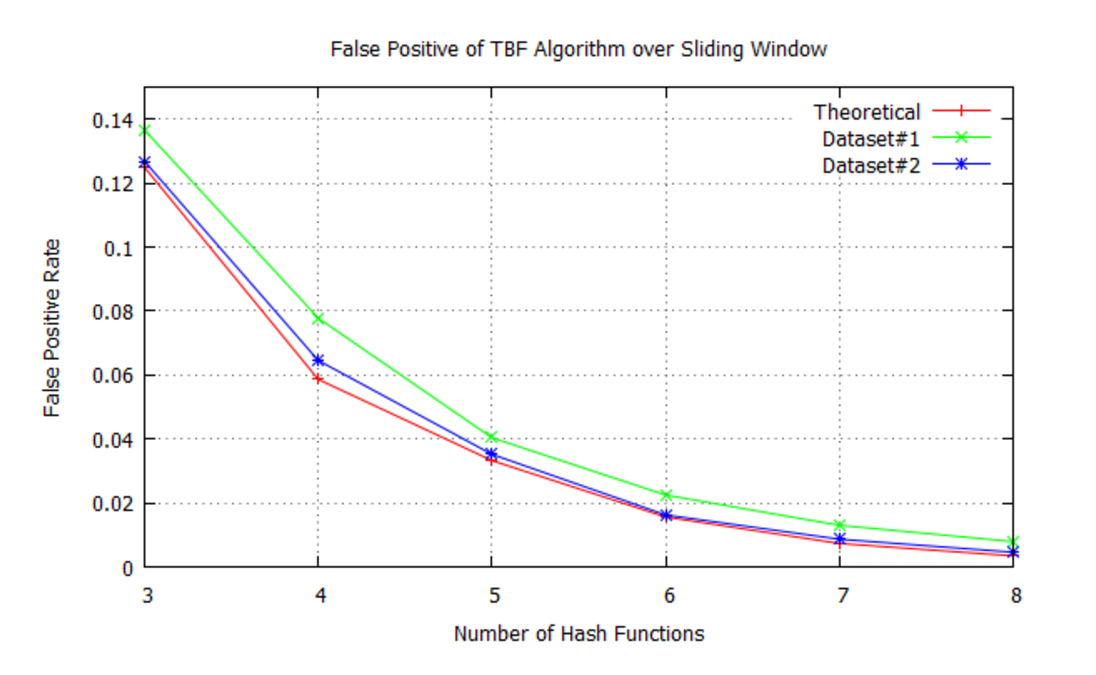
\includegraphics[height=7.5cm]{pic/result}
\caption{Experiment Results}
\label{fig:result}
\end{figure}

Figure 6 shows the three results of our experiment. We make the observation that the experimental result of TBF algorithm on Dataset\#2 is very close to the theoretical result when detecting duplicate clicks over sliding windows. It support that our implementation of TBF on sliding windows is perfect close to ideal result. Then, we can have the approximate duplicate click rate by refering to the false positive rate of our experiment result. When the entries in TBF is large enough, we can say that the false positive result is its duplicate rate.

%%%%%%%%%%%%%%%%%%%%%%%%%%%%%%%%%%%%%%%%%%%%%%%%%%%%%%%%%%%%%%%%%%
%%%%%%%%%%%%%%%%%%%%%%%%%%%%%%%%%%%%%%%%%%%%%%%%%%%%%%%%%%%%%%%%%%%%

\section{Conclusion and Future Work}\label{references}

The malicious click behavior challenges the reputation and reliance in online advertising market. 
In order to counterattack click fraud activities in the online advertising ecosystem, a framework to detect and prevent malicious clicks is necessary. At present, many ad exchange or network company own their in-house algorithms for invalid clicks detection. But there are quite few part of open framework, and also there cannot be. After the learning of many materials, we proposed our simple but feasible malicious click prevention and detection framework - ClickKeeper\footnote{Basically, I prefer the name 'Clickeeper'}.

ClickKeeper is a online and offline joint detection framework. We present the architecture including the methods of it. In the online stage, restricted timing and space efficient requires high-efficiency data structure and rule-based filtering algorithms on click streams. Through the online filtering stage, most obvious fraudulent activities can be prevent from entering into the click logs. In this paper, we have a deep introduce into the application of the TBF(timing Bloom Filter) in our online duplicate detection stage. We simulate the click stream on sliding windows and implement the TBF to detect duplicate. In our expirement, we analysis the false positive rate and its influnced parameters. The results on the synthetic and real world click log data verify our assumption, by the way, make a clear vision on the duplicate rate of the Yahoo! click log data. 


There are far more works to be done under our framework. In future work, we will extend the framework to long-term detection from every step in the online advertising serving. Another future work is to evaluate kinds of classifiers fit the situation and make a reasonable strategy for classifier choosing and result blending. We could also improved the duplication detection part by more efficient algorithms. Especially, in many cases, N click duplicate detection in a short time is more practical than one click duplicate detection. 

%\begin{thebibliography}{4}
%
%\bibitem{jour} Smith, T.F., Waterman, M.S.: Identification of Common Molecular
%Subsequences. J. Mol. Biol. 147, 195--197 (1981)
%
%\bibitem{lncschap} May, P., Ehrlich, H.C., Steinke, T.: ZIB Structure Prediction Pipeline:
%Composing a Complex Biological Workflow through Web Services. In: Nagel,
%W.E., Walter, W.V., Lehner, W. (eds.) Euro-Par 2006. LNCS, vol. 4128,
%pp. 1148--1158. Springer, Heidelberg (2006)
%
%\bibitem{book} Foster, I., Kesselman, C.: The Grid: Blueprint for a New Computing
%Infrastructure. Morgan Kaufmann, San Francisco (1999)
%
%\bibitem{proceeding1} Czajkowski, K., Fitzgerald, S., Foster, I., Kesselman, C.: Grid
%Information Services for Distributed Resource Sharing. In: 10th IEEE
%International Symposium on High Performance Distributed Computing, pp.
%181--184. IEEE Press, New York (2001)
%
%\bibitem{proceeding2} Foster, I., Kesselman, C., Nick, J., Tuecke, S.: The Physiology of the
%Grid: an Open Grid Services Architecture for Distributed Systems
%Integration. Technical report, Global Grid Forum (2002)
%
%\bibitem{url} National Center for Biotechnology Information, \url{http://www.ncbi.nlm.nih.gov}
%
%\end{thebibliography}

\bibliographystyle{splncs}
\bibliography{ref}		% expects file "myrefs.bib"

\end{document}
